\section{Computation and certification with \CosCert}\label{sec:computation}

\subsection{A certified distribution function for \texorpdfstring{$T_H$}{T\_H}}
Write $F_H(c)=P(T_H\le c)=P(Z^2-c\,D_{\SN}\le0)$. By \cref{prop:coords}, $D_{\SN}=W_J+R_J$ with
$W_J=\sum_{k\le J}\Lambda_k^2/(k\pi)^2$, a quadratic form in the $(J+1)$-dimensional Gaussian vector
$(Z,\Lambda_1,\dots,\Lambda_J)$ with closed-form covariance, and the remainder $R_J\ge0$ of \cref{thm:eig}. Let
$X_J=Z^2-cW_J$ and $\bar\mu_J=\min(\tau_J,\bar c_J)$.

\begin{theorem}[Certified enclosure]\label{thm:certificate}
Let $\frac12\le H<1$, $c>0$, $J\ge1$, $t>0$, and
$s_{\mathrm{hi}}=\tau_J+2\sqrt{\bar\mu_J\tau_Jt}+2\bar\mu_Jt$, $s_{\mathrm{lo}}=\max(0,\tau_J-2\sqrt{\bar\mu_J\tau_Jt})$. Then
\[P(X_J\le c\,s_{\mathrm{lo}})-e^{-t}\;\le\;F_H(c)\;\le\;P(X_J\le c\,s_{\mathrm{hi}})+e^{-t}.\]
For every $x$, every $\Delta>0$ and every tilt $\vartheta\in(0,\frac12)$, the exceedance probability satisfies
\[\big|P(X_J>x)-S_{\Delta,K}(x)\big|\le\epsilon_\Delta^+(x)+\epsilon_\Delta^-+\epsilon_K,\]
where $S_{\Delta,K}$ is the sum of the first $K$ terms of the tilted midpoint sum $S_\Delta$ of the inversion integral,
$\epsilon_\Delta^\pm$ bound the upper and lower aliases of $S_\Delta$ and $\epsilon_K$ the omitted terms, all given
explicitly in the proof (\cref{app:proofs}) and \cref{app:certificate}; hence $P(X_J\le x)=1-P(X_J>x)$ is enclosed by an interval of the same width. With $x=c\,s_{\mathrm{lo}}$ and
$x=c\,s_{\mathrm{hi}}$ the two statements together give a computable enclosure of $F_H(c)$.
\end{theorem}

The theorem reduces the infinite-dimensional problem to a finite one with explicit, rigorous error terms: the
remainder enters only through $\tau_J$, which is a closed form, and $\bar c_J$ from \cref{thm:eig}; the remainder's
dependence on $(Z,W_J)$ never needs to be known. The finite problem is solved in ball arithmetic \citep{Joh17}.
The characteristic function of $X_J$ is evaluated without an eigendecomposition of the $(J+1)$-dimensional covariance:
the odd cosine coordinates are uncorrelated with the rest (\cref{prop:coords}c), so the determinant factorises into an odd block, an even block and a scalar Schur
complement carrying $Z$; each factor is evaluated as a head block of up to $128$ coordinates, diagonalised approximately in floating point and
corrected by an exact similarity transformation in ball arithmetic, and a tail block bounded through its trace,
Frobenius norm and couplings.
The principal branch of every square root is the correct one on the whole strip $0\le\operatorname{Re}z<\frac12$
(\cref{lem:branch}): the scalar factor carrying $Z$, $r(z)=1-2z\,s^\top(I+2zB)^{-1}s$, has
$\operatorname{Im}r(\vartheta+\mathrm it)=-2t\sum_js_j^2/|1+2zb_j|^2$ and $r(\vartheta)\ge1-2\vartheta$, so it never meets the
cut $(-\infty,0]$. Critical values follow by bracketing: if the certified lower bound of $F_H$ at $q^+$ exceeds $p$ and
the certified upper bound at $q^-$ falls below $p$, then $q_p\in[q^-,q^+]$.

All production values use $J=16384$ and $t=25$, so that each of the two exceptional probabilities is $e^{-25}<1.4\times10^{-11}$.
The protocol fixed these choices before production, after a benchmark over $J=512,\dots,16384$ (\cref{fig:certificate}b):
the width of the enclosure decreases like $J^{-1/2-2H}$, as \cref{prop:rate} below predicts (the measured local slopes
differ from $-\frac12-2H$ by at most \pthree{e1-slope-maxdev} for $J\le8192$), and at $J=16384$ it is at most
\pthree{e1-width-max-16384} in probability. For $H\ge0.95$ the last doubling of $J$ gains less, because the
finite-dimensional radius, which does not decrease with $J$, is reached. The tilted inversion
($\vartheta=\frac14$) needs \pthree{e1-tilt-node-ratio-min}--\pthree{e1-tilt-node-ratio-max} times fewer nodes than the
untilted one at the same accuracy.

The rate of the enclosure, and what it depends on, can be stated precisely.

\begin{proposition}[Width of the enclosure]\label[proposition]{prop:rate}
Let $\frac12\le H<1$, $c>0$, $t\ge1$, $J_0\ge4$, and let $\alpha_2\ge\alpha_3\ge\alpha_4$ be the second to fourth largest
eigenvalues of the covariance of $(\Lambda_k/(k\pi))_{k\le J_0}$. For every $J\ge J_0$ with $\tau_J\ge4\bar c_Jt$, the
interval of the first statement of \cref{thm:certificate} has width
\[w_J\le c\bar f\big(4\sqrt{\bar c_J\tau_Jt}+2\bar c_Jt\big)+2e^{-t},\qquad
\bar f=\frac1{2\pi}\int_{\mathbb R}\prod_{i=2}^4\big(1+4c^2\alpha_i^2s^2\big)^{-1/4}\dd s<\infty .\]
Since $\tau_J\asymp J^{-2H}$ and $\bar c_J\asymp J^{-1-2H}$, $w_J-2e^{-t}=O(\sqrt t\,J^{-1/2-2H})$, where
$t=\log(1/p)$ for a failure probability $p$. The computed enclosure adds the numerical radii of \cref{app:certificate},
which do not decrease with $J$, and a quantile bracket has width close to $w_J/f_H(q)$.
\end{proposition}

\begin{figure}[tbp]\centering
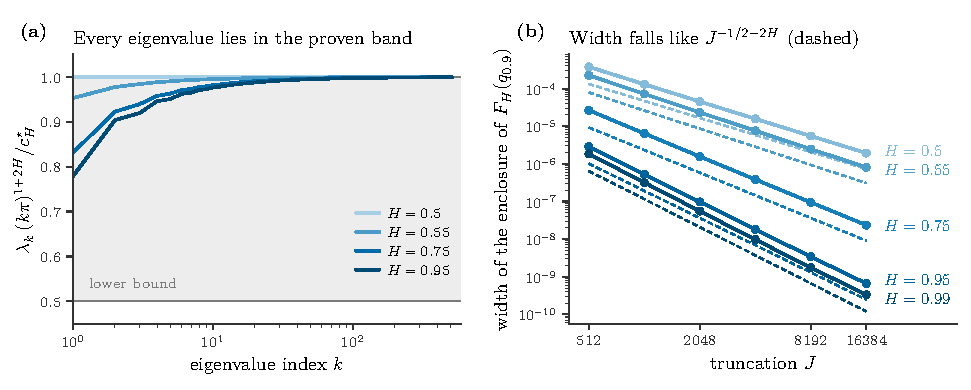
\includegraphics[width=\textwidth]{fig6_certificate.pdf}
\caption{Spectrum and certificate of the fractional Brownian bridge. (a)~Eigenvalues relative to the upper bound of
\cref{thm:eig} (Galerkin, $J=2048$); the lower bound is $\frac12$. (b)~Width of the certified enclosure of $F_H$ at the
$90\,\%$ quantile against $J$; dashed: slope $-\frac12-2H$ (\cref{prop:rate}), offset for visibility.}\label{fig:certificate}
\end{figure}

\subsection{Computational methods on identical targets}\label{sec:methods}
We compared \pthree{e5-n-impl} implementations and modes of \pthree{e5-n-methods} distinct methods for generalized
chi-square probabilities on four targets: a fixed-$m$ limit (T1, $m=8$, $H=0.8$), an EWC limit (T2, $B=16$, $H=0.8$),
the exact finite-sample law of $T_n$ at $n=1000$ under ARFIMA$(0,0.2,0)$ (T3), and the limit law of $T_H$ at $H=0.75$
(T4). Every method received the same weights. The covariance of the fixed-smoothing coordinates is a shared input;
beyond it, each method is charged the spectral step it needs, the certified enclosure its enclosure of the weights and
the double-precision methods a Cholesky factorisation and the eigenvalues of the ratio form, which depend on the cutoff.
Against a certified enclosure $[L,U]$ a computed value $v$ has a true error in
$[\operatorname{dist}(v,[L,U]),\max(|v-L|,|v-U|)]$, and we report this interval; on T3 the reference is the computed
exact law of \cref{prop:exactn}(b), which the Imhof and Bromwich implementations confirm to $10^{-13}$. A method used
outside its documented domain is run and labelled but not compared: the approximation of \citet{LTZ09} is documented
for non-negative definite forms, and all four targets are indefinite. The R methods for positive forms, those of
\citet{Hal83} and \citet{BE88} (HBE) and \citet{LPB00} (LPB4) as implemented by \citet{BA16}, and the saddlepoint and
\citet{Sat46} options of the survey package \citep{Lum04}, are applied to the negative part of the form and integrated
over the positive one by adaptive quadrature; a $64$-node Gauss--Hermite rule, which does not resolve the kink of that
integrand, changes their values by up to \pthree{e5-gh-maxdiff-pp}\,pp.

\begin{figure}[tbp]\centering
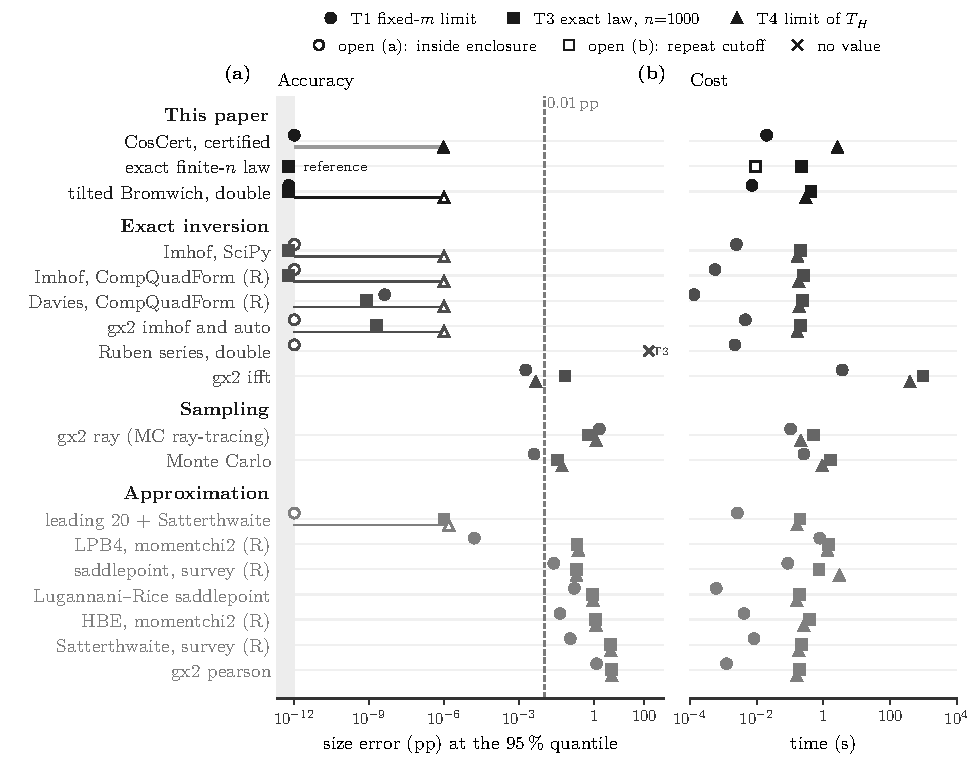
\includegraphics[width=\textwidth]{fig5_methods.pdf}
\caption{Accuracy and cost of computational methods on identical targets (T1, T3, T4; \cref{sec:methods}). (a)~Size
error at the $95\,\%$ quantile; open markers: upper bounds (value inside the certified enclosure); grey bars: certified
half-widths; shaded: double-precision floor. (b)~Wall-clock time including each method's spectral step.}\label{fig:methods}
\end{figure}

Three conclusions follow. First, on the low-rank targets T1 and T2 every exact inversion method, Imhof's integral in
three implementations (SciPy, the R package of \citet{DL10}, and the \texttt{imhof} and \texttt{auto} modes of
\citet{Das25}), Davies' algorithm, Ruben's series and our tilted Bromwich rule, has error at most
\pthree{e5-T12-exact-maxerr} in probability at a cost below \pthree{e5-T12-exact-maxs}\,s, and the certified enclosure,
of width \pthree{e5-T12-cert-width}, costs \pthree{e5-T12-cert-s}\,s. Second, the approximations are not accurate enough
for critical values. At the $5\,\%$ level the saddlepoint approximation of \citet{Kuo99} errs by up to
\pthree{e5-lr-err-pp}\,pp in size, HBE by \pthree{e5-hbe-err-pp}, the saddlepoint option of survey by
\pthree{e5-svsaddle-err-pp}, LPB4 by \pthree{e5-lpb4-err-pp} and Satterthwaite's two-moment approximation by
\pthree{e5-satt-err-pp}\,pp; Pearson's three-moment approximation (the \texttt{pearson} mode of \citet{Das25}) errs by
\pthree{e5-3mom-T1-pp}\,pp on T1 and returns the probability $1$ on T3 and T4, an error of
\pthree{e5-approx-maxerr-pp}\,pp. A hybrid of the type studied by \citet{CL19}, which keeps the $20$ largest weights exactly and replaces
the others by a two-moment scaled chi-square with fractional degrees of freedom, is accurate to
\pthree{e5-lead20-err} in probability on every target. Third, for the long-memory targets the cost is the spectral step.
On T3 the exact law of \cref{prop:exactn}(b) pays \pthree{e5-T3-setup-s}\,s once, for one Cholesky factorisation and one
eigendecomposition, and then \pthree{e5-T3-query-s}\,s per cutoff, whereas a method that needs the eigenvalues of the
cutoff-dependent ratio form pays \pthree{e5-T3-eig-s}\,s for them at every cutoff (\pthree{e5-T3-imhof-s}\,s in all with
Imhof's integral). For one cutoff the costs are comparable; over \pthree{e5-amort-m} cutoffs they are
\pthree{e5-amort-ours-s}\,s and \pthree{e5-amort-imhof-s}\,s, with agreement to \pthree{e5-amort-maxdiff}. The
\texttt{ifft} mode of \citet{Das25} took \pthree{e5-T3-ifft-s}\,s on T3 and was less accurate, and on T4 with $J=2048$
it exceeded the available memory; the \texttt{ray} mode took \pthree{e5-T4-ray2048-s}\,s there. On T4, Imhof's
integral on the $J=512$ cosine coordinates, with the remainder replaced by its mean, lies inside the certified
enclosure, of width \pthree{e5-T4-ref-width}, so its error is at most \pthree{e5-T4-galerkin-err}; it takes
\pthree{e5-T4-galerkin-s}\,s against \pthree{e5-T4-cert-s}\,s for the certified evaluation at $J=16384$, including the
construction of the system. We recommend it whenever a guarantee is not needed, and use the certificate to confirm it.
All times are wall-clock times on one machine (\pthree{e5-env}, single-threaded linear algebra) and indicate orders of
magnitude only.
